%!TEX root = main.tex

\section{Effective Algorithms for Unconstrained Optimization}
All of the methods we have explored so far (Newton-Raphson, Secant methods, Steepest descent) offer sound algorithms to compute local extrema of real-valued functions $f \colon \field{R}^d \to \field{R}$. They do have some pros and cons.  
\begin{itemize}
	\item The method of Steepest descent produces non-increasing iterations.
	\item In order to obtain new approximations on each Steepest descent iteration, we have to solve many different one-dimensional optimizations, each of them offering their own computational issues. 
	\item Both Newton-Raphson and Secant methods offers faster sequences, but we cannot always guarantee convergence.  
	\item Another drawback of both Newton-Raphson and Steepest descent is the fact that we do need expressions for function itself, its gradient and Hessian matrix.  
	\item The recurrence formulas of Broyden's method are simple, and require only evaluations of the function itself.
\end{itemize}

The goal of this section is precisely gathering the best properties of the previous methods, so we may craft new methods with all the advantages, but none of the shortcomings.  

\separator

Given a function $f \colon \field{R}^d \to \field{R}$ with continuous first partial derivatives, and a given initial guess $\x_0 \in \field{R}^d$, we search for a recursive formula to approximate a minimum of $f$.  We request that this formula has the form
\begin{equation*}
\x_{n-1} = \x_n + t_n \w_n,
\end{equation*}
with positive parameters $t_n > 0$, and vectors $\w_n$ satisfying the following criteria:
\begin{description}
	\item[Non-increasing sequences] $f(\x_{n+1}) < f(\x_n)$ whenever $\gradient{f}(\x_n) \neq 0$. 

	\noindent This is achieved by requiring the vectors $\omega_n$ to have an angle larger than $\pi/2$ with respect to $\gradient{f}(\x_n)$:
	\begin{equation}
	\langle \w_n , \gradient{f}(\x_n) \rangle < 0.\label{Criterion2}
	\end{equation}
	Why does this work? Consider at each step $n \in \field{N}$ the restriction $\varphi_n(t)=f\big( \x_n + t \w_n \big)$ of $f$ over the line $\x_n + t \w_n$ with $t>0$.  We have then $\varphi_n'(0) = \langle \gradient{f}(\x_n), \w_n \rangle < 0$ (a decreasing function near $t=0$).  We have a guaranteed value $t_n > 0$ (that could be very small) that give us a point $\x_{n+1} = \x_n + t_n \w_n$ with $f(\x_{n+1}) < f(\x_n)$.
	\item[Control over length of steps] The steps $t_n$ are not \emph{too short, nor too long}.

	\noindent This is achieved by picking first $0 < \mu < \lambda < 1$ and forcing vectors $\omega_n$ that satisfy
	\begin{gather}
	\langle \w_n , \gradient{f}(\x_{n+1}) - \lambda \gradient{f} (\x_n) \rangle > 0 \label{Criterion3}\\
	f(\x_{n+1}) \leq f(\x_n) + \mu t_n \langle \w_n \gradient{f}(\x_n) \rangle \label{Criterion4}
	\end{gather}
	if this is at all possible.
	\item[Easy to compute] Duh!
\end{description}

\separator

Is it possible to create a iteration satisfying these criteria?  The following result gives us a condition that helps in this regard:

\begin{theorem}[Wolfe]\label{theorem:Wolfe}\index{Theorem!Wolfe}
Suppose that $f \colon \field{R}^d \to \field{R}$ is a real-valued function with continuous partial derivatives.  Assume there exists $M \in \field{R}$ so that $f(x) \geq M$.  Let $\lambda, \mu$ be fixed numbers satisfying $0 < \lambda < \mu < 1$.  If $\w_n$, $\x_n \in \field{R}^d$ satisfy Criterion \eqref{Criterion2}, then there exist real numbers $a_n, b_n$ such that $0 \leq a_n < b_n$ and
\begin{enumerate}
	\item Criterion \eqref{Criterion3} is satisfied for any choice of $t_n \in (0, b_n)$, and
	\item Criterion \eqref{Criterion4} is satisfied for any choice of $t_n \in (a_n, b_n)$.
\end{enumerate}
\end{theorem}

\begin{remark}
For a proof, see \cite[Theorem 3.3.1]{peressini1988mathematics}.
\end{remark}

Using these principles, we are going to see two constructions based upon secant methods: the DFP and BFGS methods.

\subsection{The DFP Method}\index{DFP method|see{Davidon-Fletcher-Powell method}}\index{Davidon-Fletcher-Powell method}
The Davidon-Fletcher-Powell method is is one of the earliest and most effective secant methods. Its effectiveness stems from the fact that the method simultaneously generates conjugate directions and constructs an approximation of the inverse of the Hessian matrix. In each step, the inverse of the Hessian is updated by the sum of two symmetric rank 1 matrices. For this reason, it is referred to as a “rank 2” correction procedure. It is also called a “variable metric method”.

To minimize $f \colon \field{R}^d \to \field{R}$, select an initial guess $\x_0$ and an initial \emph{positive definite} matrix $\boldsymbol{A}_0$.  If $\x_n$ and $\boldsymbol{A}_n$ have been computed, then 
\begin{enumerate}
	\item Find $t_n>0$ so that $\x_{n+1} = \x_n - t_n \overbrace{\boldsymbol{A}_n \cdot \transpose{\gradient{f}(\x_n)}}^{\w_n}$ satisfies criteria \eqref{Criterion2}, \eqref{Criterion3} and \eqref{Criterion4}.
	\item Update
	\begin{equation}\label{equation:DFP}
	\boldsymbol{A}_{n+1} = \boldsymbol{A}_n + \frac{\boldsymbol{d}_n \otimes \boldsymbol{d}_n}{\langle \y_n, \boldsymbol{d}_n \rangle } - \frac{\boldsymbol{A}_n \transpose{\y}_n \otimes \boldsymbol{A}_n \transpose{\y}_n }{\quadratic{\boldsymbol{A}_n}(\y_n)}
	\end{equation}
	with $\boldsymbol{d}_n = \x_{n+1}-\x_n= t_n\w_n$, and $\y_n = \gradient{f}(\x_{n+1}) - \gradient{f}(\x_n)$.
\end{enumerate}

\begin{remark}
Unlike in the general Broyden's method, all the matrices $\boldsymbol{A}_n$ constructed in \eqref{equation:DFP} are positive definite. 
\end{remark}

\subsection{The BFGS method}\index{BFGS method|see{Broyden-Fletcher-Goldfarb-Shanno method}}\index{Broyden-Fletcher-Goldfarb-Shanno method}
The DFP method was soon superseded by the BFGS method, which is its dual (interchanging the roles of $\boldsymbol{d}_n$ and $\y_n$).

Different parts of this method were devised by Broyden, Fletcher, Goldfarb and Shanno independently in 1969.  Their communications were sent as manuscripts between March and June of 1969, and reviewed between October 1969 and January 1970.  They were all published in 1970.  Each of these mathematicians derived similar formulas using different techniques (see \cite{broyden1970convergence}, \cite{fletcher1970new}, \cite{goldfarb1970family}, \cite{shanno1970conditioning} and \cite{shanno1970optimal})

To minimize $f \colon \field{R}^d \to \field{R}$, select an initial guess $\x_0$ and an initial \emph{positive definite} matrix $\boldsymbol{A}_0$.  If $\x_n$ and $\boldsymbol{A}_n$ have been computed, then
\begin{enumerate}
	\item Find $t_n>0$ so that $\x_{n+1} = \x_n - t_n \overbrace{\boldsymbol{A}_n^{-1} \cdot \transpose{\gradient{f}(\x_n)}}^{\w_n}$ satisfies criteria \eqref{Criterion2}, \eqref{Criterion3} and \eqref{Criterion4}.
	\item Update
	\begin{equation}\label{equation:BFGS}
	\boldsymbol{A}_{n+1} = \boldsymbol{A}_n + \frac{\y_n \otimes \y_n}{\langle \boldsymbol{d}_n, \y_n \rangle } - \frac{\boldsymbol{A}_n \transpose{\boldsymbol{d}}_n \otimes \boldsymbol{A}_n \transpose{\boldsymbol{d}}_n }{\quadratic{A_n} (\boldsymbol{d}_n) }
	\end{equation}
	with $\boldsymbol{d}_n = \x_{n+1}-\x_n= t_n\w_n$, and $\y_n = \gradient{f}(\x_{n+1}) - \gradient{f}(\x_n)$.
\end{enumerate}

\begin{remark}
Like in the DFP method, all the matrices $\boldsymbol{A}_n$ constructed in \eqref{equation:BFGS} are positive definite.  For a proof, see e.g.~\cite[Theorem 3.5.2]{peressini1988mathematics}.
\end{remark}

\begin{example}\index{scipy}\index{BFGS method}
In Python there is an implementation of BFGS in the libraries \scipy\texttt{.optimize}: the routine \texttt{fmin\_bfgs()}.  The following session illustrates how to use this method to approximate the minimum of the Rosenbrock function $\mathcal{R}_{1,1}$  with an initial guess $(x_0, y_0)=(-2,2)$

\begin{minted}[frame=single, fontsize=\footnotesize, linenos, mathescape]{python}
import numpy as np, matplotlib.pyplot as plt 
from scipy.optimize import fmin_bfgs

# Rosenbrock $\mathcal{R}_{1,1}$ function
def R(x): 
	return (1.0-x[0])**2 + (x[1] - x[0]**2)**2

# its Jacobian/gradient $\gradient{\mathcal{R}_{1,1}}$
def jacR(x): 
	return np.array([-2.*(1.-x[0])-4.*x[0]*(x[1]-x[0]**2), 
                          2.*(x[1]-x[0]**2)])

# Setup for diagrams. 
x = np.linspace(-3,3)
y = np.linspace(-3,3)
X,Y = np.meshgrid(x,y)
\end{minted}

We call \texttt{fmin\_bfgs} with the function and its gradient (with the option \texttt{fprime=}), the initial guess $(-2,2)$, and activate the option \texttt{retall=True} that offers the complete list of iterations obtained by the algorithm.

% We may not need this if we make modifications prior to this point.  Check often
% \newpage

\begin{minted}[frame=single,fontsize=\footnotesize, mathescape]{python}
>>> result = fmin_bfgs(R, [-2.,2.], fprime=jacR, retall=True)
Optimization terminated successfully.
         Current function value: 0.000000
         Iterations: 12
         Function evaluations: 15
         Gradient evaluations: 15

>>> plt.figure(figsize=(8,8));
... plt.axes(aspect='equal');
... plt.contour(X, Y, (1-X)**2+(Y-X**2)**2, \
...             colors='k', \
...             levels=[0.2,0.8,1,1.4,1.78,2.23,4,5.4,8,13,32,64]);
... plt.plot(x, x**2, 'r--');
... plt.xlim(-3, 3);
... plt.ylim(-1, 3);
... plt.plot([p[0] for p in result[1]], [p[1] for p in result[1]], 'b.-');
... plt.title("Convergence to critical point:\nBFGS on Rosenbrock");
... plt.show()
\end{minted}

\begin{figure}[ht!]
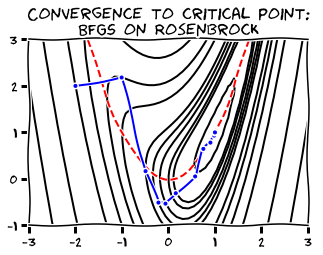
\includegraphics[width=0.65\linewidth]{images/bfgs.png}
\caption{The BFGS method: Rosenbrock function}
\label{figure:BFGS}
\end{figure}
\end{example}






